

\documentclass[12pt, a4paper]{article}


\usepackage{fancyhdr, enumerate}
\usepackage{amssymb}
\usepackage{geometry, amsmath, amsfonts, float, graphicx}
\usepackage{gensymb}
\usepackage{hyperref, listings}
\usepackage{matlab-prettifier}
\usepackage{caption}
\def\Z{\mathbb Z}
\geometry{
	top=0.9in,           
	inner=0.6in,
	outer=0.6in,
	bottom=2in,
	tmargin= 10ex,       
	headsep=0.6cm,          
}
\pagestyle{fancy}

\fancyhead{}
\fancyfoot{}

\fancyhead[L]{Bioen 316 AC \\Homework 7\\ June 6, 2019}
\fancyhead[R]{Skyler Hallinan\\ hallisky@uw.edu \\ 1732227}

\lstMakeShortInline[style=Matlab-editor]"
\begin{document}
\vspace*{-3mm}
\section*{Problem 1} 
In the past few weeks, you have analyzed a second-order band-pass RLC circuit to apply
before sampling, applied an FIR filter to extract EEG beta waves, and seen MATLAB’s IIR
filter design tool. For this homework, use MATLAB to compare the behavior of these three
filter types, all with cutoff frequencies of 0.5 and 50 Hz. For the digital filters, choose a
sampling frequency that can handle 120 Hz noise, i.e. the first harmonic of 60 Hz. \\ \\
\textbf{Answer: } \\ 
Our comparison of the three filtering methods is shown in this plot:
\begin{figure}[H]
\centering
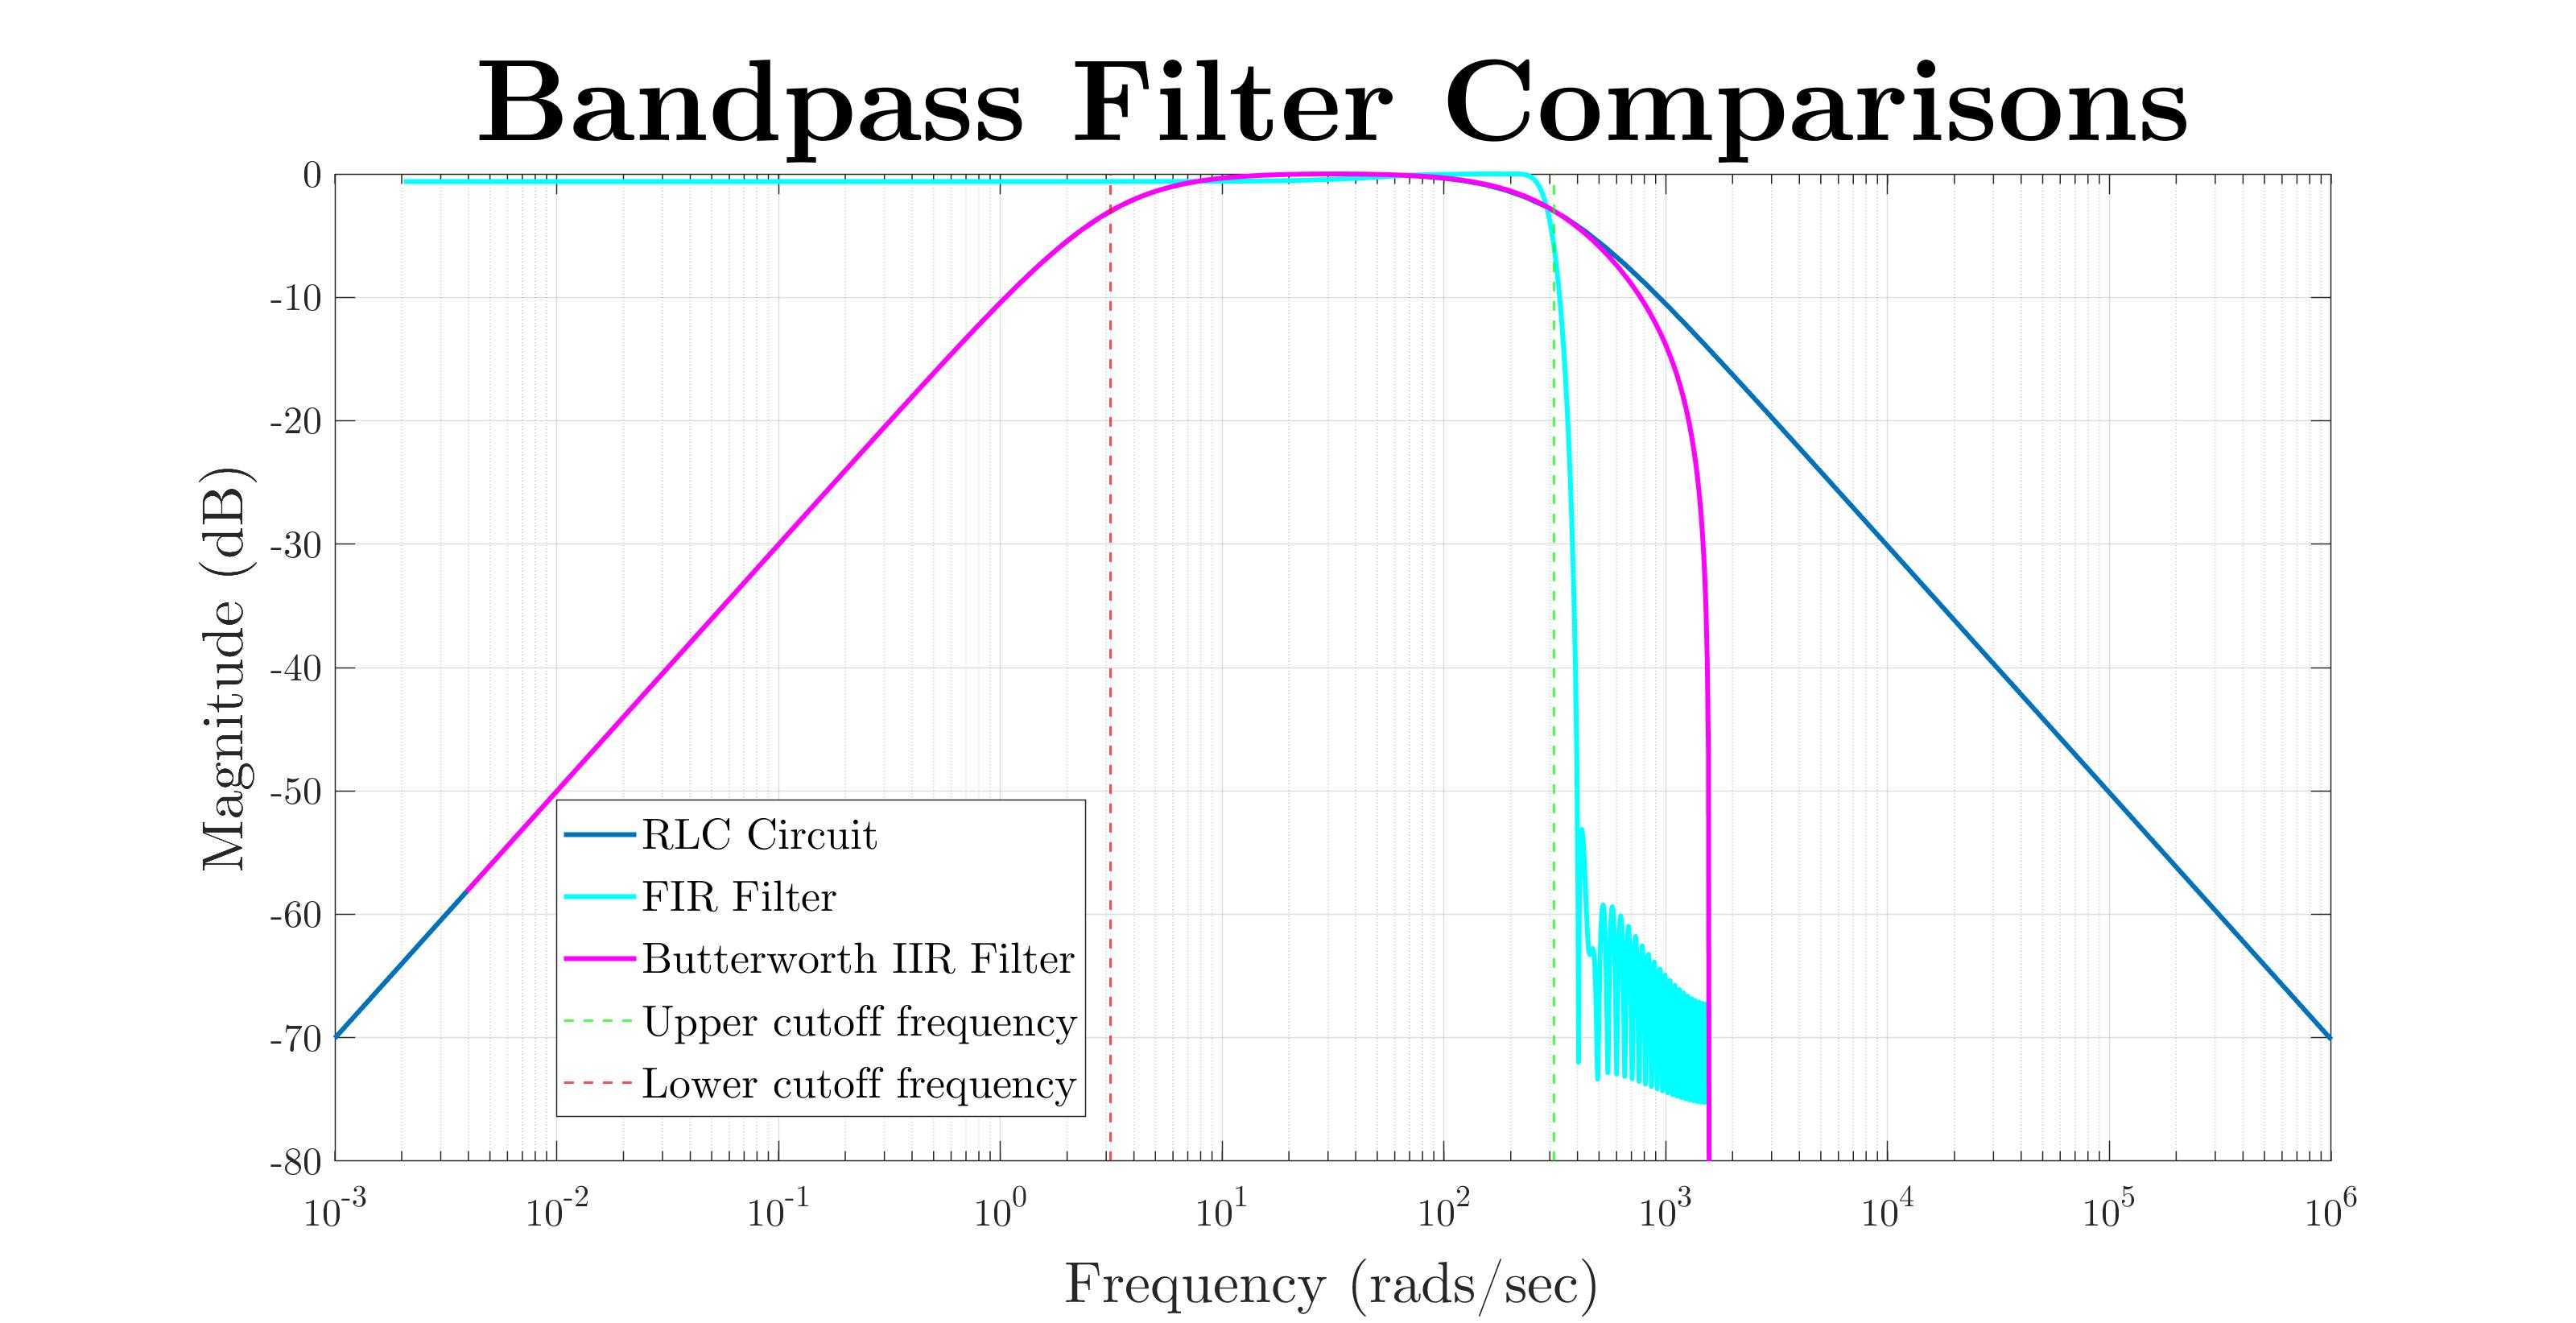
\includegraphics[width=\textwidth]{bpf}
\caption{Bandpass filter comparisons of three varying methods}
\end{figure}
\noindent We conducted the filtering in radians per second ($\omega$). We calculated our low pass and high pass cutoff frequencies of the band pass filter, $\omega_{low}$ and $\omega_{high}$, to be $\pi$ and $100 \pi$ respectively. We also had the following equations: 
\begin{align*}
\omega_{h i}=+\alpha+\sqrt{\alpha^{2}+\omega_{0}^{2}}, \quad \omega_{l o w}=-\alpha+\sqrt{\alpha^{2}+\omega_{0}^{2}}
\end{align*}
We calculated our $\alpha$ to be $\frac{99}{2} \pi$, from subtracting our equations relating our $\omega_{low}$ and $\omega_{high}$ to their $\omega_0$ and simplifying for alpha; $\alpha = \frac{\omega{high}-\omega{low}}{2} = \frac{99}{2}\pi$. Finally, we calculated our $\omega_0$ to be 10 $\pi$, found from substituting our calculated values into their equations and isolating for $\omega_0$. \\ \\
We first created an RLC filter using the general form, $G(\omega)=\frac{2 \alpha j \omega}{(j \omega)^{2}+2 \alpha j \omega+\omega_{0}^{2}}$, and inputted a variety of frequencies to create the Bode plot. Then, we created a FIR filter as in the previous homework, centering it at $\frac{101 \pi}{2}$ and applying a Hamming smoothing window. We used a sampling frequency of 500 Hz, as this was higher than 2 times the 120 Hz electrical noise that was present, so it could properly handle it. By Nyquist's Theorem, we can avoid aliasing of this frequency by choosing a sampling frequency that is sufficiently high (above 2 times that frequency), hence we chose 500 Hz. 500 Hz is more than two times greater than 120, so we do not have to worry about aliasing occurring. We also used this when we created our last filter in \textsc{Matlab}, the 2nd-order Butterworth filter. \\ \\
\noindent We see that the RLC filter performs well, giving clear bandpass filtering of our desired frequencies, with attenuation on the sides of higher or lower undesired frequencies. The Butterworth IIR filter also performs relatively well, but it has a noticeably steeper decline after the upper frequency cutoff than does the RLC filter. In addition, the RLC filter and Butterworth filter align almost perfectly on the left side (for lower frequencies). Although it seems like the RLC circuit extends more on the left side, it is just because we used different number of points/ranges for the two filters. Finally, we see that the FIR filter does not do a good job at attenuating lower frequencies. There is a horizontal line to the left of the lower cutoff frequency at a relatively low magnitude dB scale. This means the FIR filter is not attenuating low frequencies as it should be doing. However, it does filter higher frequencies (above the upper cutoff) more successfully, albeit with some oscillatory behavior.\\ \\
See the code for more annotation.
\pagebreak
\section*{\fontsize{19}{15}\selectfont Appendix A}
\subsection*{MATLAB code}
 \lstinputlisting[style=Matlab-editor]{hw7.m}
\end{document}